\begin{frame}
    \begin{center}
        {\large Experiments}
    \end{center}        
\end{frame}

\begin{frame}[t]
    \frametitle{Lotka-Volterra model}
    Two non-linear ODEs to model the interaction between prey and predator.
    \begin{align}
        \dot{x}(t) & = \alpha x(t) - \beta x(t)y(t)
        \nonumber
        \\
        \dot{y}(t) & = \delta x(t)y(t) - \gamma y(t)
        \label{eq-lotka-odes}
    \end{align}
    where 
    \begin{itemize}
        \item[] $x(t), y(t) \in \R_{\geqslant 0}$ are the populations of prey and predator at time $t$.    
        \item[] $\alpha, \beta, \delta, \gamma \in \R^+$ are the parameters controlling the dynamics.
    \end{itemize}
\end{frame}

\begin{frame}[t]
    \frametitle{Experimental setup}
    \begin{table}
        \centering
        \label{table-lotka-setup}
        \begin{tabular}{|c|c|c|c|c|c|c|c|c|}
            \hline
            $K$ & $K_{obs}$ & $t_0$ & $t_T$ & $\delta t$ & $\alpha, \beta, \delta, \gamma$ & $\dymsigmak{k}^2$  & $freq_{obs}$ \\ \hline
        2 & 2 & 0 & 2 & 0.01 & 2, 1, 1, 4 & 0.1 & 10 \\ \hline
        \end{tabular}
    \end{table}
\end{frame}

\begin{frame}[t]
    \frametitle{State estimation}
    \begin{figure}
        \centering
        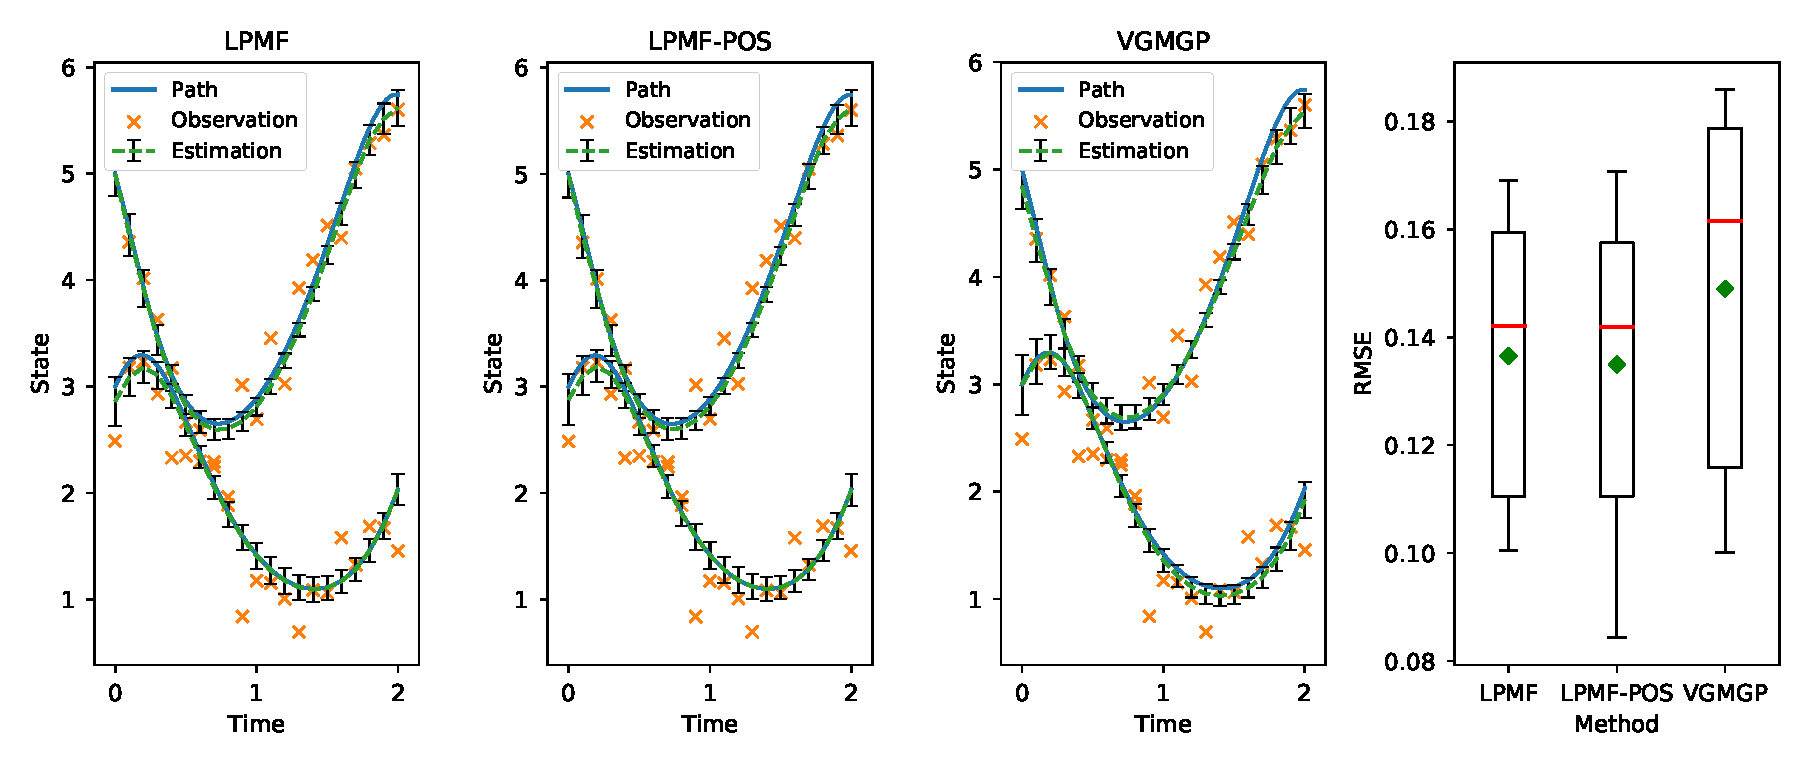
\includegraphics[width=\textwidth]{graphics/lotka-states}
        \label{fig-lotka-state}
    \end{figure}
\end{frame}

\begin{frame}[t]
    \frametitle{Parameter estimation}
    \begin{figure}
        \centering
        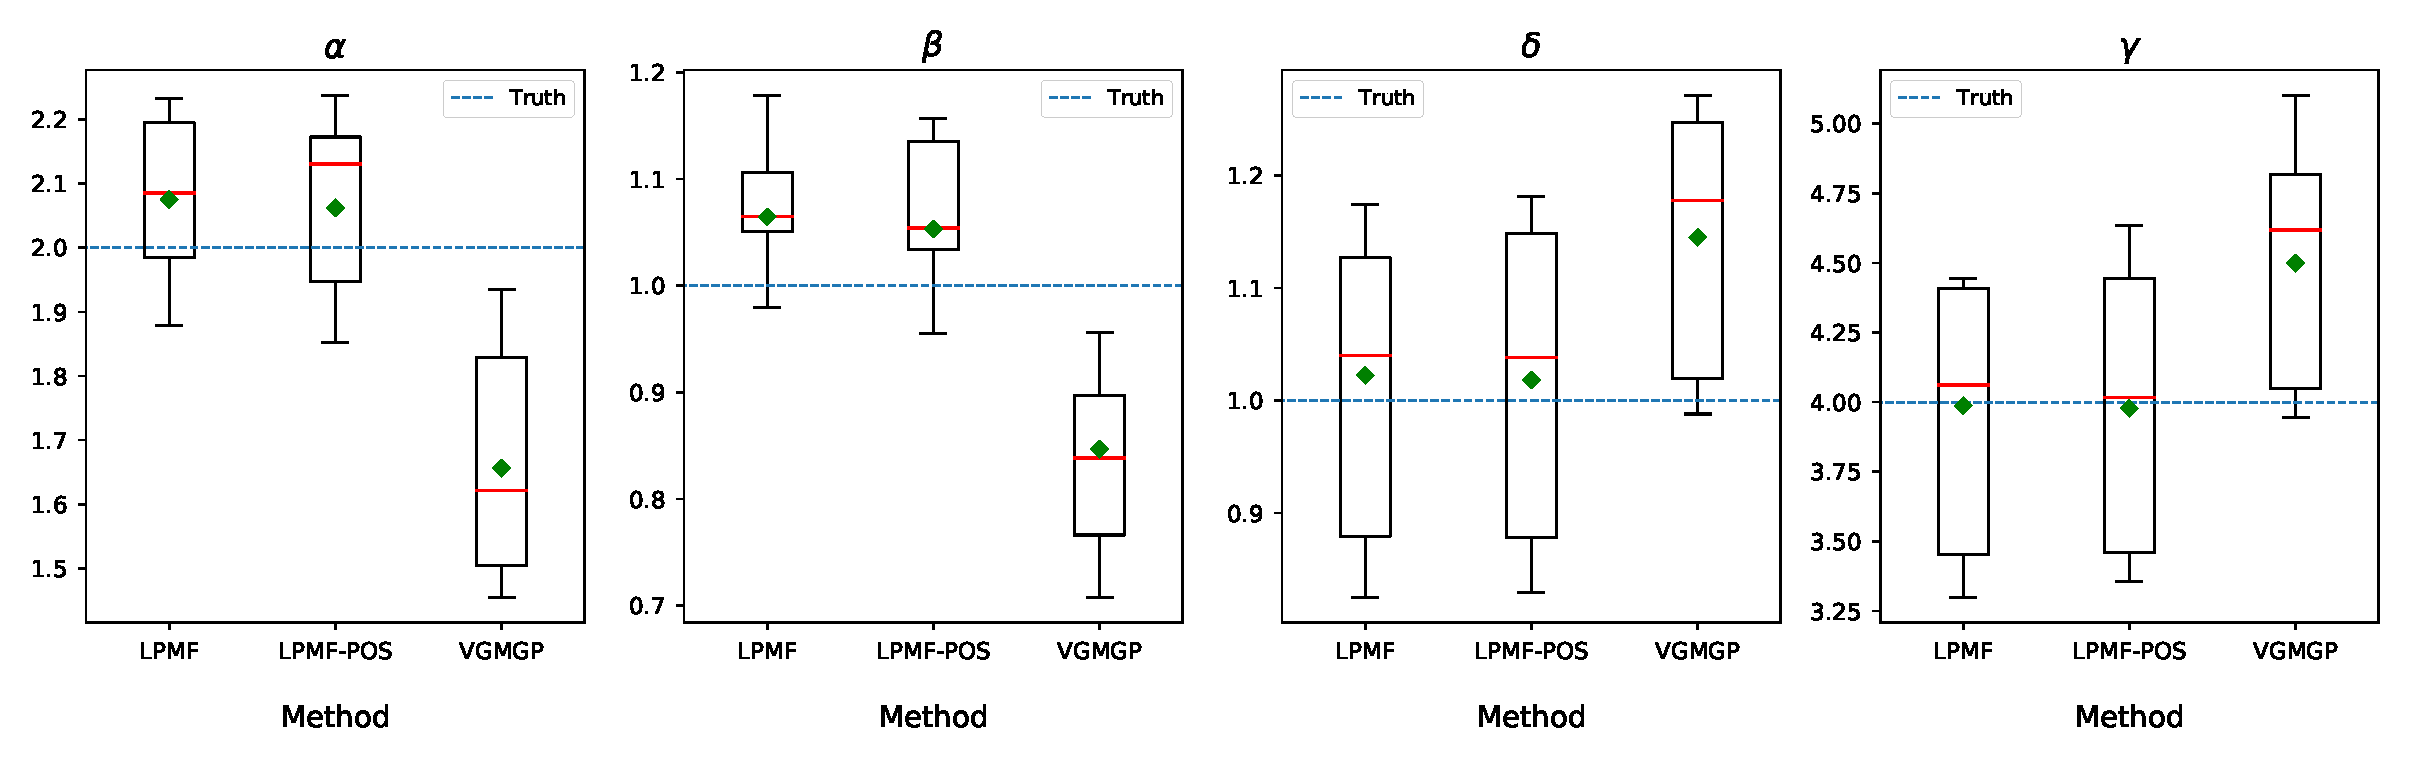
\includegraphics[width=1\textwidth]{graphics/lotka-parameters-boxplot}
        \label{fig-lotka-parameters-boxplot}
    \end{figure}
\end{frame}

\begin{frame}[t]
    \frametitle{Runtime performance}
    \begin{figure}
        \centering
        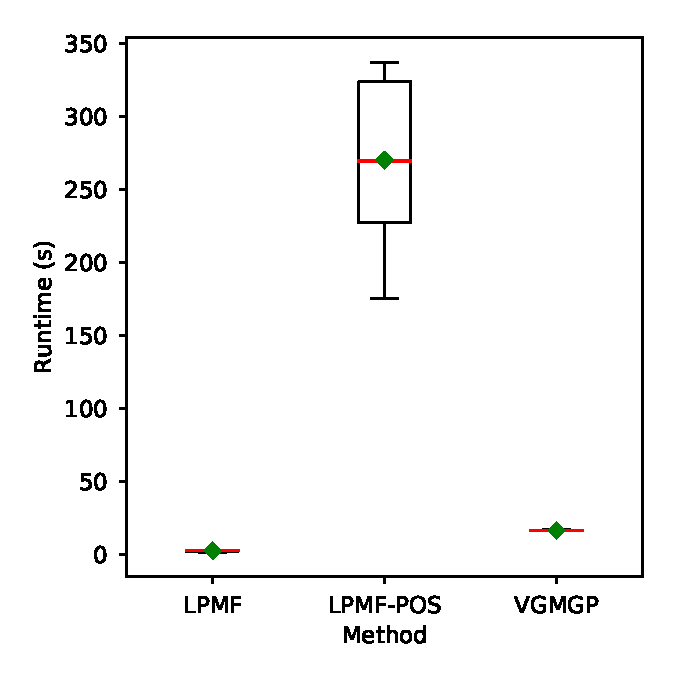
\includegraphics[width=0.45\textwidth]{graphics/lotka-runtime-boxplot}
        \label{fig-lotka-runtime-boxplot}
    \end{figure}                                       
\end{frame}

\begin{frame}[t]
    \frametitle{Positivity constraint on states}
    \begin{figure}
        \centering
        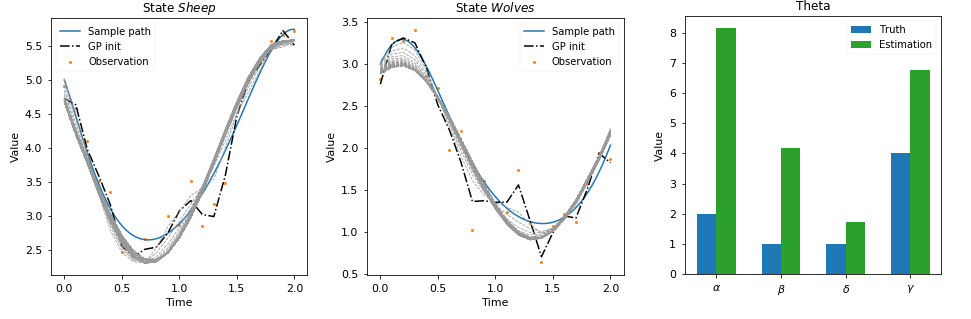
\includegraphics[width=\textwidth]{graphics/lotka-fail}
        \label{fig-lotka-fail}
    \end{figure}     
\end{frame}

\begin{frame}[t]
    \frametitle{Protein signalling transduction pathway}
    A signal transduction cascade model to describe the dynamics among protein species.
    \begin{align}
        \proteinSdt 
        & = 
        -\proteinki{1} \times \proteinS 
        -\proteinki{2} \times \proteinS \times \proteinR
        + \proteinki{3} \times \proteinRS
        \nonumber
        \\
        \proteindSdt
        & = 
        \proteinki{1} \times \proteinS    
        \nonumber
        \\
        \proteinRdt
        & =
        -\proteinki{2} \times \proteinS \times \proteinR 
        + \proteinki{3} \times \proteinRS
        + \proteinV \times \frac{\proteinRpp}{\proteinKm + \proteinRpp}
        \nonumber
        \\
        \proteinRSdt
        & =
        \proteinki{2} \times \proteinS \times \proteinR
        - \proteinki{3} \times \proteinRS
        - \proteinki{4} \times \proteinRS
        \nonumber
        \\
        \proteinRppdt 
        & =
        \proteinki{4} \times \proteinRS - \proteinV \times \frac{\proteinRpp}{\proteinKm + \proteinRpp}
    \end{align}
    where 
    \begin{itemize}
        \item[] $\proteinS, \proteindS, \proteinR, \proteinRS, \proteinRpp \ \in \R_{\geqslant 0}$ are the concentrations of proteins. 
        \item[] $\proteinki{1}, \proteinki{2}, \proteinki{3}, \proteinki{4}, \proteinKm, \proteinV \in \R^+$ are kentic parameters
    \end{itemize}
\end{frame}

\begin{frame}[t]
    \frametitle{Experimental setup}
    \begin{table}
    \centering
    \label{table-protein-setup}
    \begin{tabular}{|c|c|c|c|c|c|c|c|c|}
    \hline
    $K$ & $K_{obs}$ & $t_0$ & $t_T$ & $\delta t$ & $k_1, k_2, k_3, k_4, V, Km$ & $\dymsigmak{k}^2$ \\ \hline
    5 & 4 & 0 & 100 & 0.05 & 0.07, 0.6, 0.05, 0.3, 0.017, 3 & 0.01\\ \hline
    \end{tabular}
    \end{table}    
    
    \vspace{\baselineskip}
    The observations, in total 15, are collected at time points 0, 1, 2, 4, 5, 7, 10, 15, 20, 30, 40, 50, 60, 80 and 100.
\end{frame}

\begin{frame}[t]
    \frametitle{State estimation}
    \begin{figure}
        \centering
        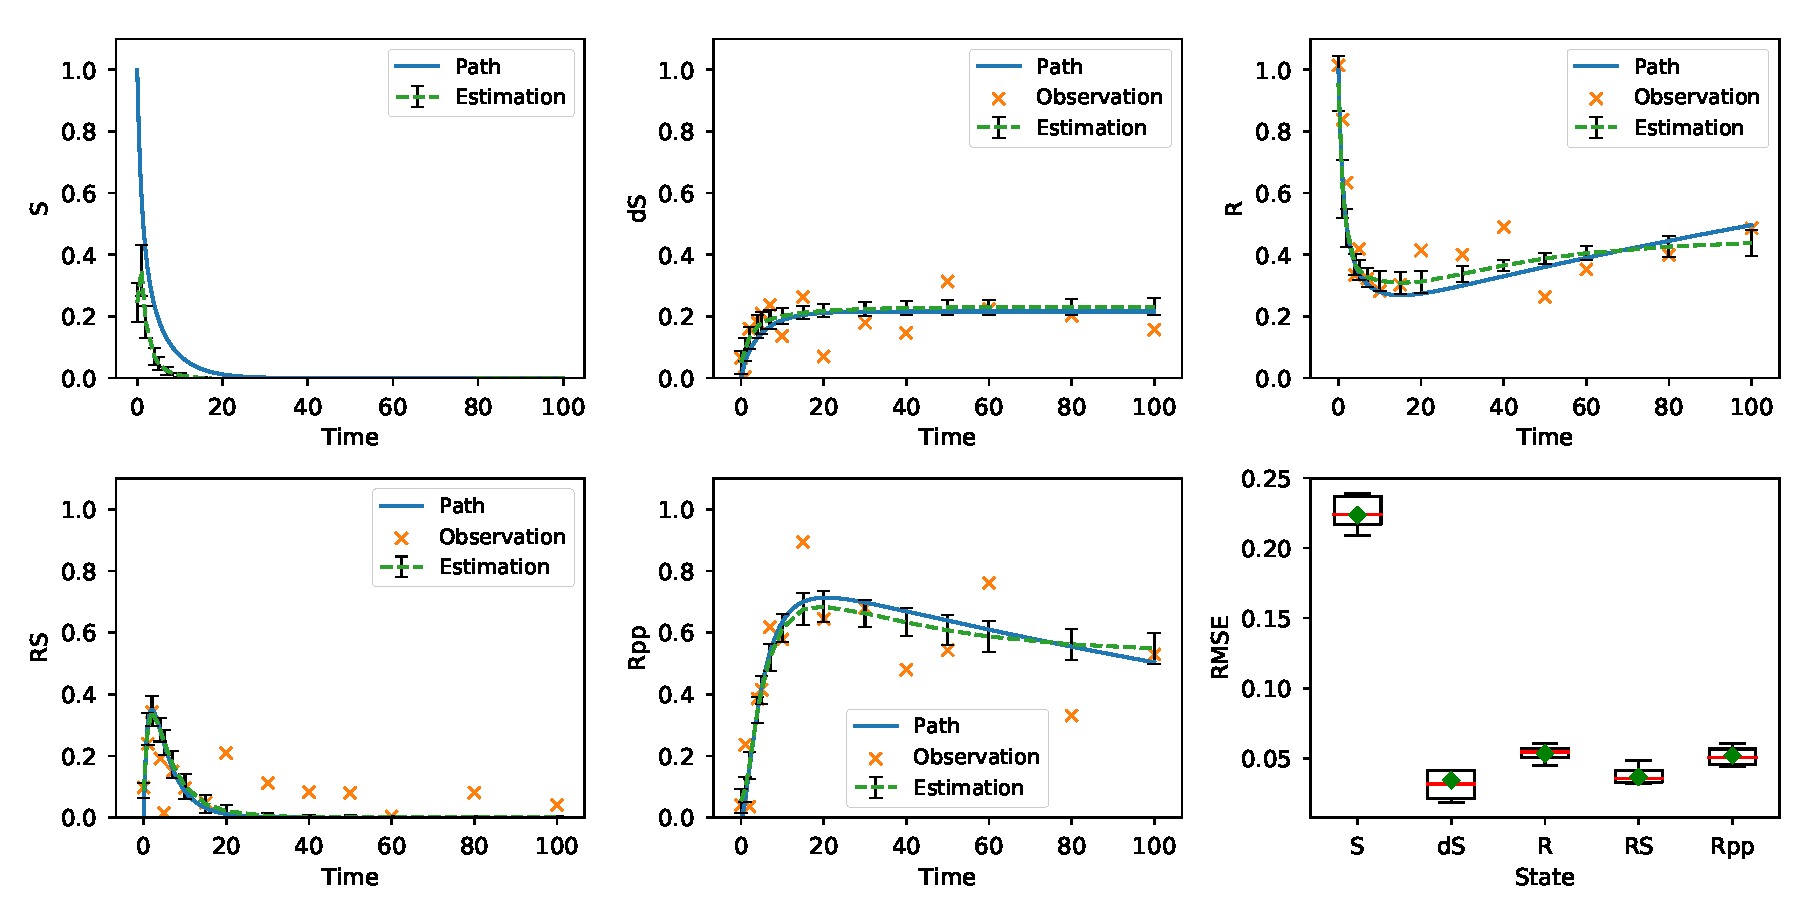
\includegraphics[width=0.9\textwidth]{graphics/protein-states-without-km-partial}
        \label{fig-protein-states-partial-without-km}
    \end{figure}
\end{frame}

\begin{frame}[t]
    \frametitle{Parameter estimation}
    \begin{figure}
        \centering
        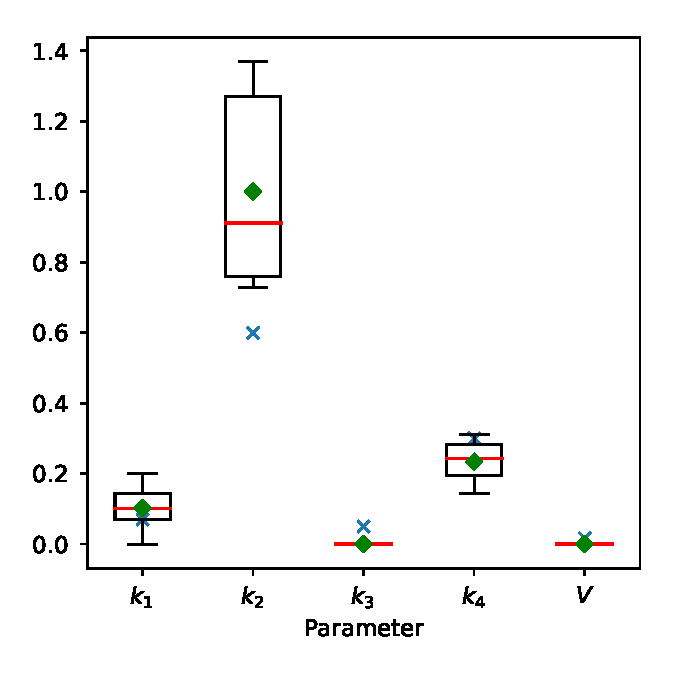
\includegraphics[width=0.4\textwidth]{graphics/protein-parameters-without-km-partial}
        \label{fig-protein-parameters-partial-without-km}
    \end{figure}            
\end{frame}

\begin{frame}[t]
    \frametitle{Lorenz 96 model}
    A minimalistic weather forecast model.
    A $K$-dimensional deterministic Lorenz 96 dynamical system is defined for $k = \mrange{1}{K}$, state-wise as follows:
    \begin{align}
        \dymdxktn{k}{}
         & = (\dymxktn{k+1}{} - \dymxktn{k-2}{})\dymxktn{k-1}{} - \dymxktn{k}{} + F
        \label{eq-lorenz-96-drift}
    \end{align}
    where
    \begin{align}
        \dymxktn{-1}{} & = \dymxktn{K-1}{}
        \nonumber
        \\
        \dymxktn{0}{} & = \dymxktn{K}{}
        \nonumber
        \\
        \dymxktn{K+1}{} & =\dymxktn{1}{}        
        \nonumber
    \end{align}
    \begin{align}
        F \in \R \text{ controls the behavior of the system}
    \end{align}
\end{frame}

\begin{frame}[t]
    \frametitle{Experimental setup}
    \begin{table}
        \centering
        \label{table-lorenz-96-setup}
        \begin{tabular}{|c|c|c|c|c|c|c|c|c|}
        \hline
        $K$ & $K_{obs}$ & $t_0$ & $t_T$ & $\delta t$ & $F$ & $\dymsigmak{k}^2$  & $\sderhoq{k}^2$ & $freq_{obs}$ \\ \hline
        500 & 325 (65\%) & 0 & 4 & 0.01 & 8 & 1 & 4 & 8 \\ \hline
        \end{tabular}
    \end{table}
\end{frame}

\begin{frame}[t]
    \frametitle{State estimation}
    \begin{figure}
        \centering
        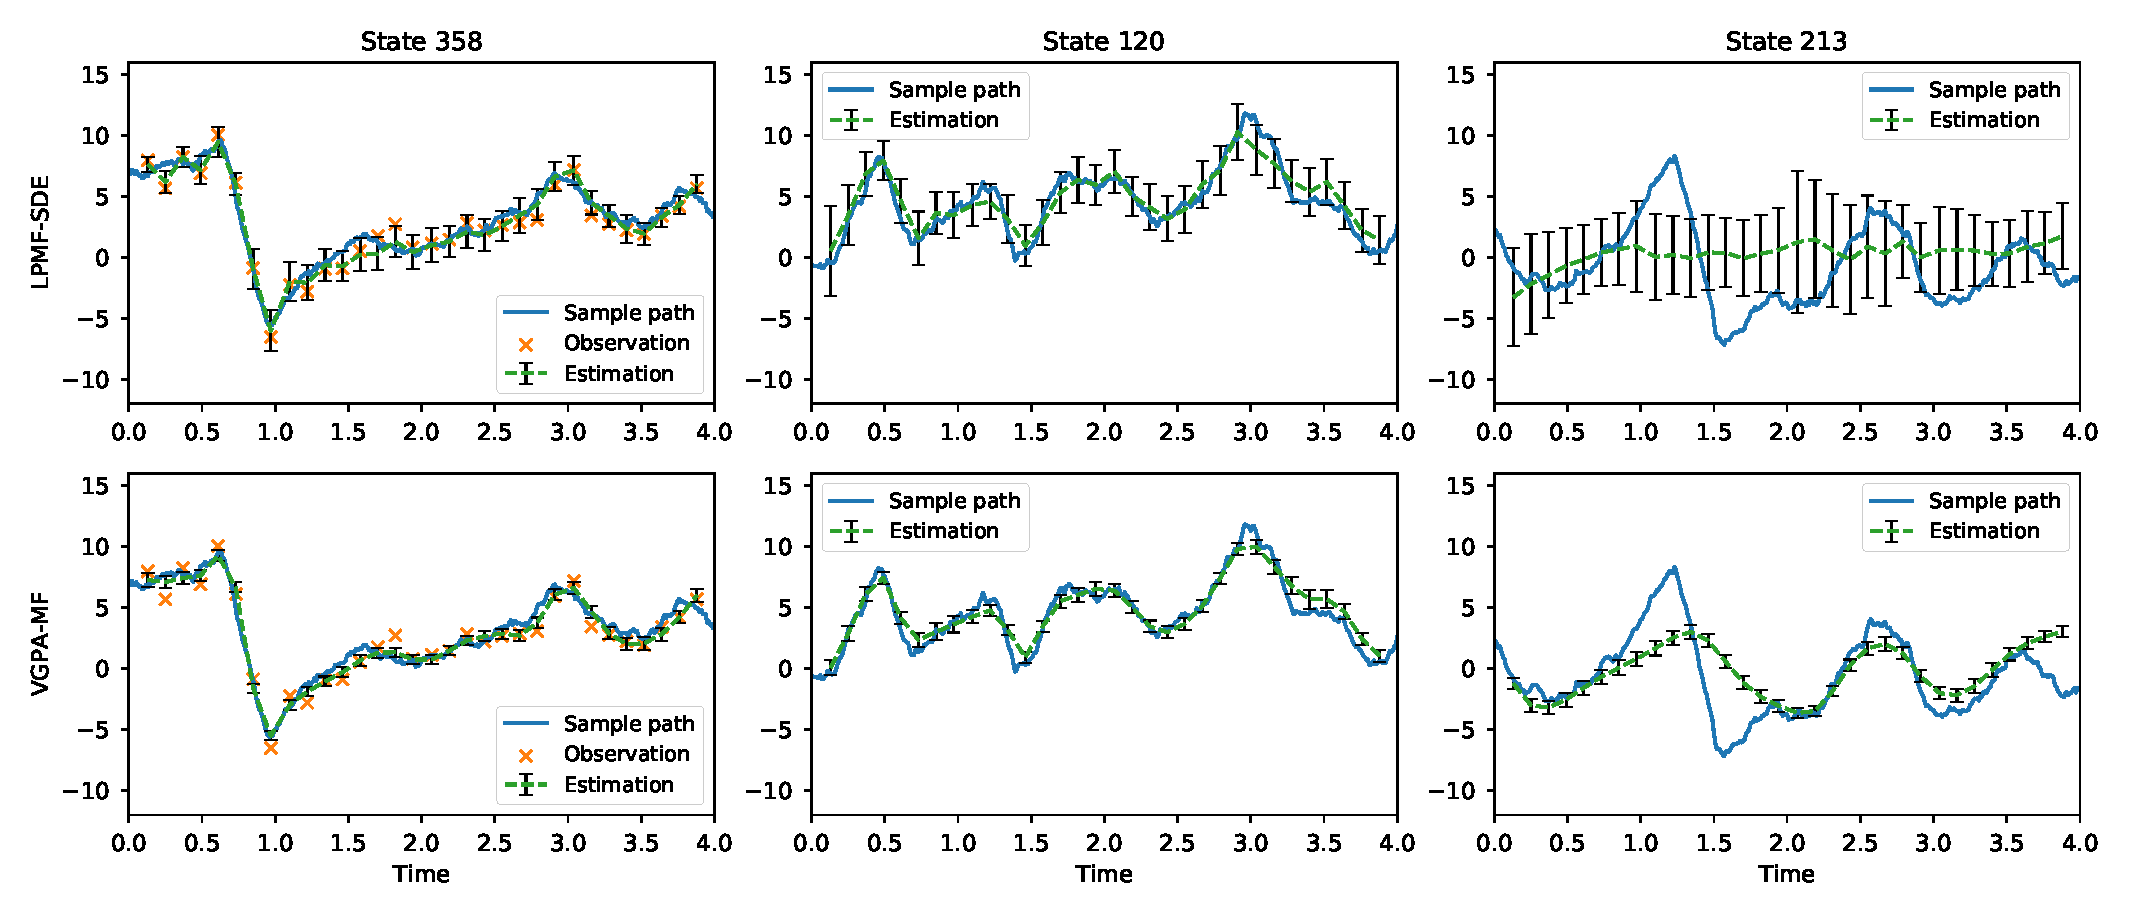
\includegraphics[width=\textwidth]{graphics/lorenz-96-states}
        \label{fig-lorenz-96-states}
    \end{figure}
\end{frame}

\begin{frame}[t]
    \frametitle{State estimation}
    \begin{figure}
        \centering
        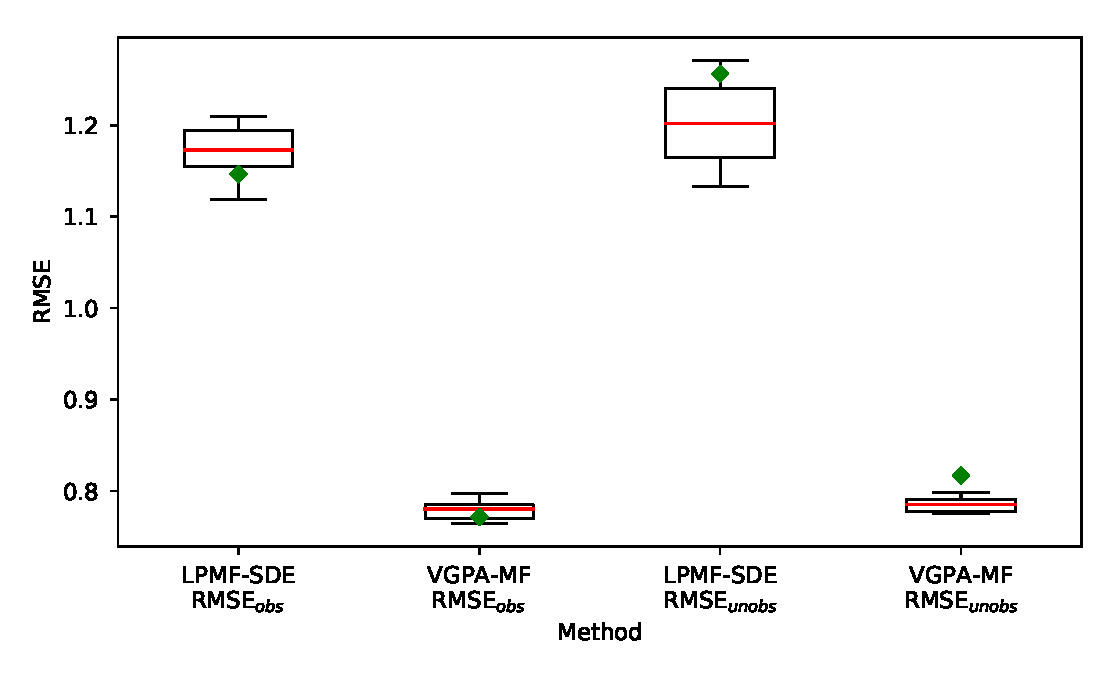
\includegraphics[width=0.7\textwidth]{graphics/lorenz-96-states-boxplot}    
        \label{fig-lorenz-96-state-boxplot}
    \end{figure}
\end{frame}

\begin{frame}[t]
    \frametitle{Parameter estimation}
    \begin{figure}
        \centering
        \begin{subfigure}[b]{0.32\textwidth}
            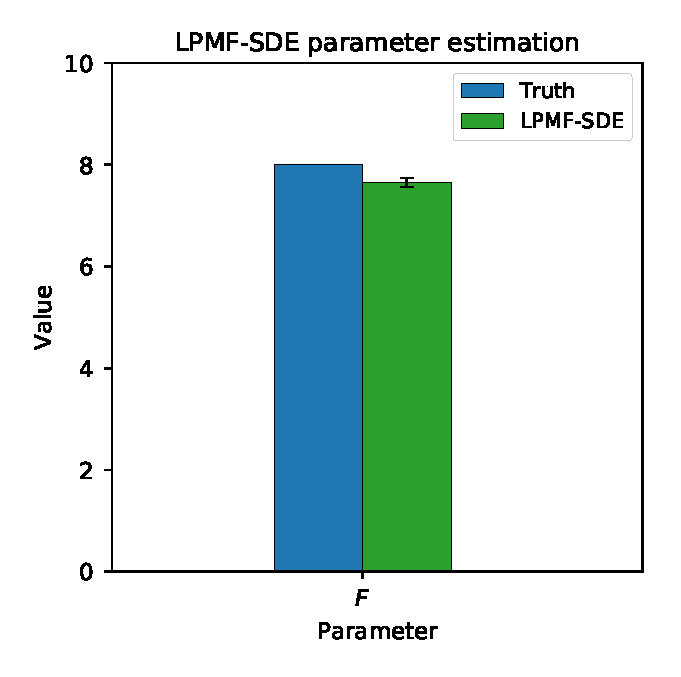
\includegraphics[width=\linewidth]{graphics/lorenz-96-parameters}
            \label{fig-lorenz-96-parameters}
        \end{subfigure}
        \begin{subfigure}[b]{0.32\textwidth}
            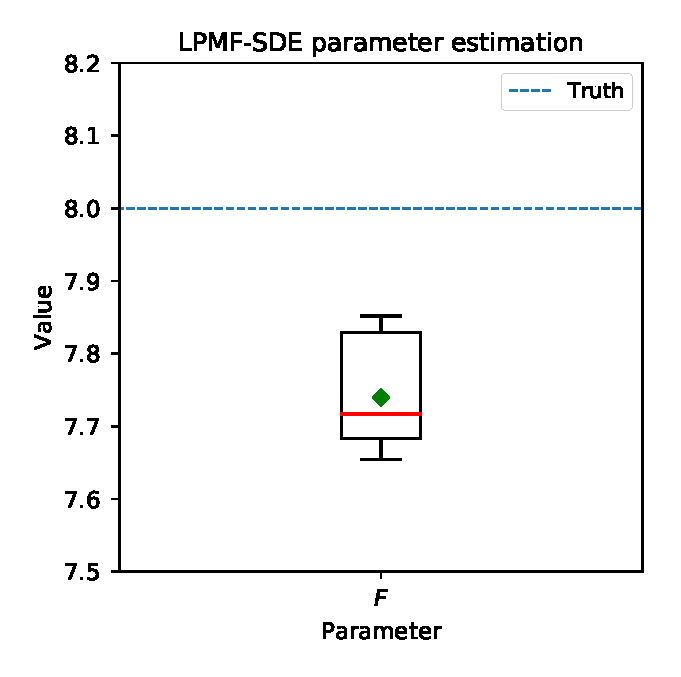
\includegraphics[width=\linewidth]{graphics/lorenz-96-parameters-boxplot}
            \label{fig-lorenz-96-parameters-boxplot}
        \end{subfigure}
        \begin{subfigure}[b]{0.32\textwidth}
            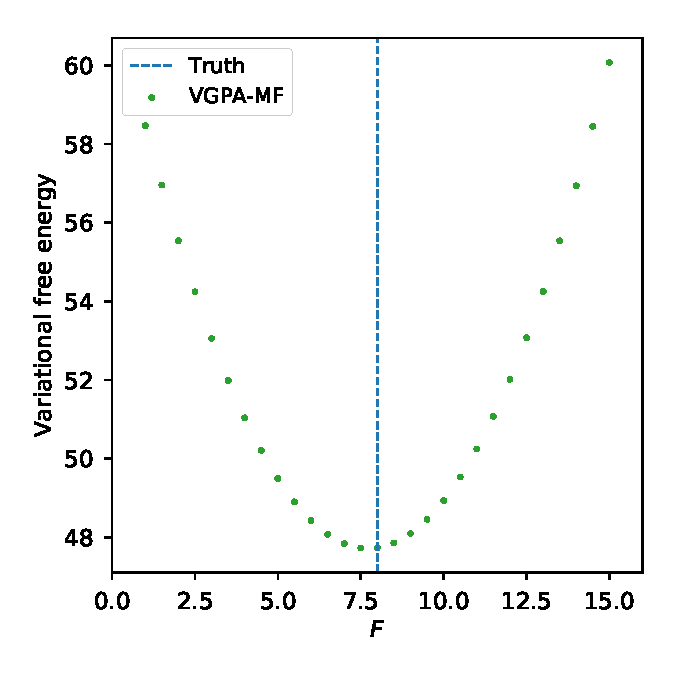
\includegraphics[width=\textwidth]{graphics/lorenz-96-parameters-grid-search}
            \label{fig-lorenz-96-parameters-grid-search}
        \end{subfigure}
        \label{fig-lorenz-96-parameters-group}    
    \end{figure}
\end{frame}

\begin{frame}[t]
    \frametitle{Runtime performance}
    \begin{figure}
        \centering
        \begin{subfigure}[b]{0.42\textwidth}
            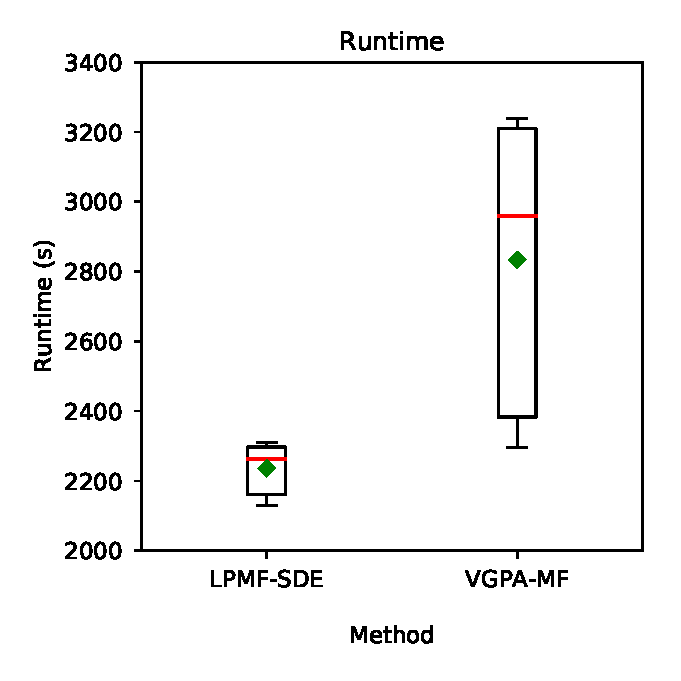
\includegraphics[width=\textwidth]{graphics/lorenz-96-runtime-boxplot}
            \label{fig-lorenz-96-runtime-boxplot}
        \end{subfigure}
        \begin{subfigure}[b]{0.56\textwidth}
        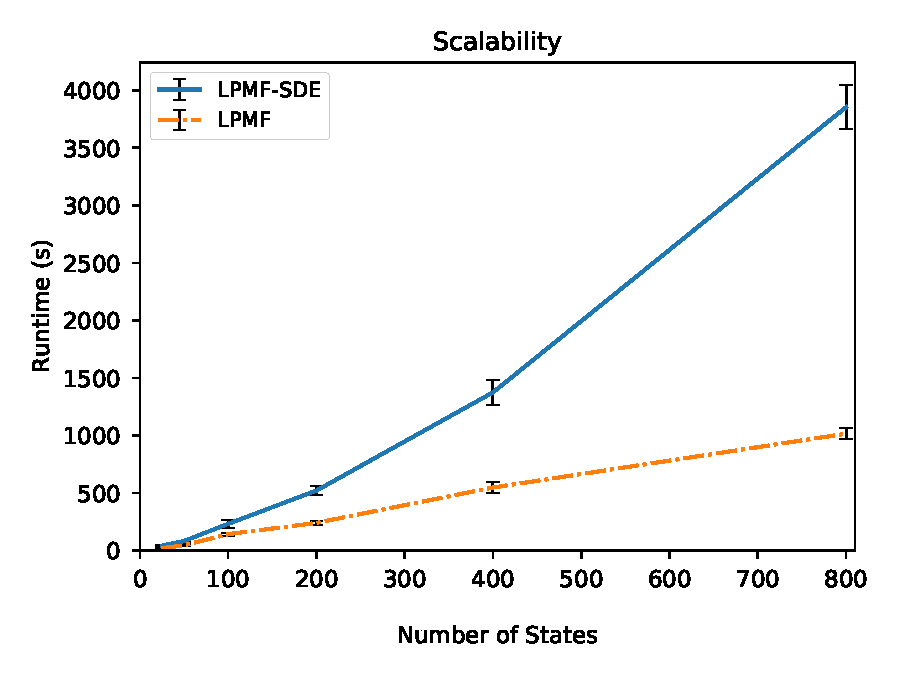
\includegraphics[width=\textwidth]{graphics/lorenz-96-scalability}
        \label{fig-lorenz-96-scalability}
        \end{subfigure}  
    \end{figure}    
\end{frame}

\begin{frame}[t]
    \frametitle{Lorenz 63 model}
    Low dimensional mathematical model for thermal convection in the atmosphere.
    The vector field of the deterministic Lorenz 63 is defined as follows:
    \begin{align}
        \dymf
        & =
        \begin{bmatrix}
            \dot{x}(t)
            \\ 
            \dot{y}(t)
            \\
            \dot{z}(t)
        \end{bmatrix}
        =
        \begin{bmatrix}
            \sigma(y(t) - x(t))
            \\
            x(t)(\rho - z(t)) - y(t)
            \\
            x(t)y(t) - \beta z(t)
        \end{bmatrix}
        \label{eq-lorenz-63-odes}
    \end{align}
    where
    \begin{itemize}
        \item[] $\dymx = [x(t), y(t), z(t)]^\top \in \R^3$ is the state vector.
        \item[] $\dymtheta = [\sigma, \rho, \beta]^\top \in \R^3$ is the parameter vector
    \end{itemize}
\end{frame}

\begin{frame}[t]
    \frametitle{Experimental setup}
    \begin{table}
    \centering
    \label{table-lorenz-63-setup}
    \begin{tabular}{|c|c|c|c|c|c|c|c|c|}
    \hline
    $K$ & $K_{obs}$ & $t_0$ & $t_T$ & $\delta t$ & $\sigma, \rho, \beta$ & $\dymsigmak{k}^2$  & $\sderhoq{k}^2$ & $freq_{obs}$ \\ \hline
    3 & 3 or 2 & 0 & 20 & 0.01 & $10, 28, \frac{8}{3}$ & 2 & 10 & 5 \\ \hline
    \end{tabular}
    \end{table}    
\end{frame}

\begin{frame}[t]
    \frametitle{Sample path}
    \begin{figure}
        \centering
        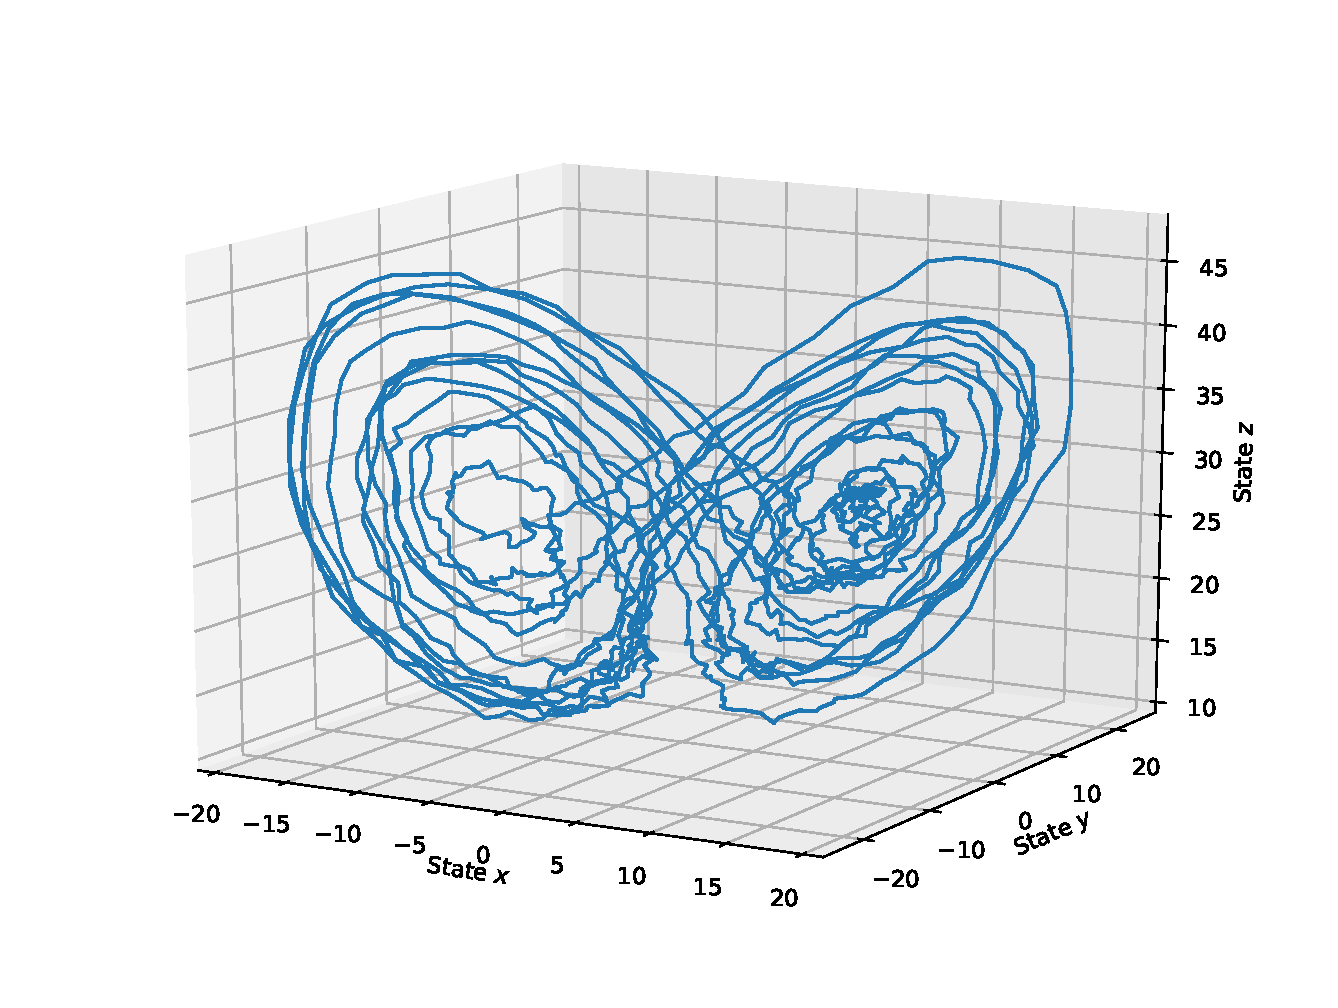
\includegraphics[width=0.6\textwidth]{graphics/lorenz-63-sample-path}
        \label{fig-lorenz-63-sample-path}
    \end{figure}    
\end{frame}

\begin{frame}[t]
    \frametitle{State estimation}
    \begin{figure}
        \centering
        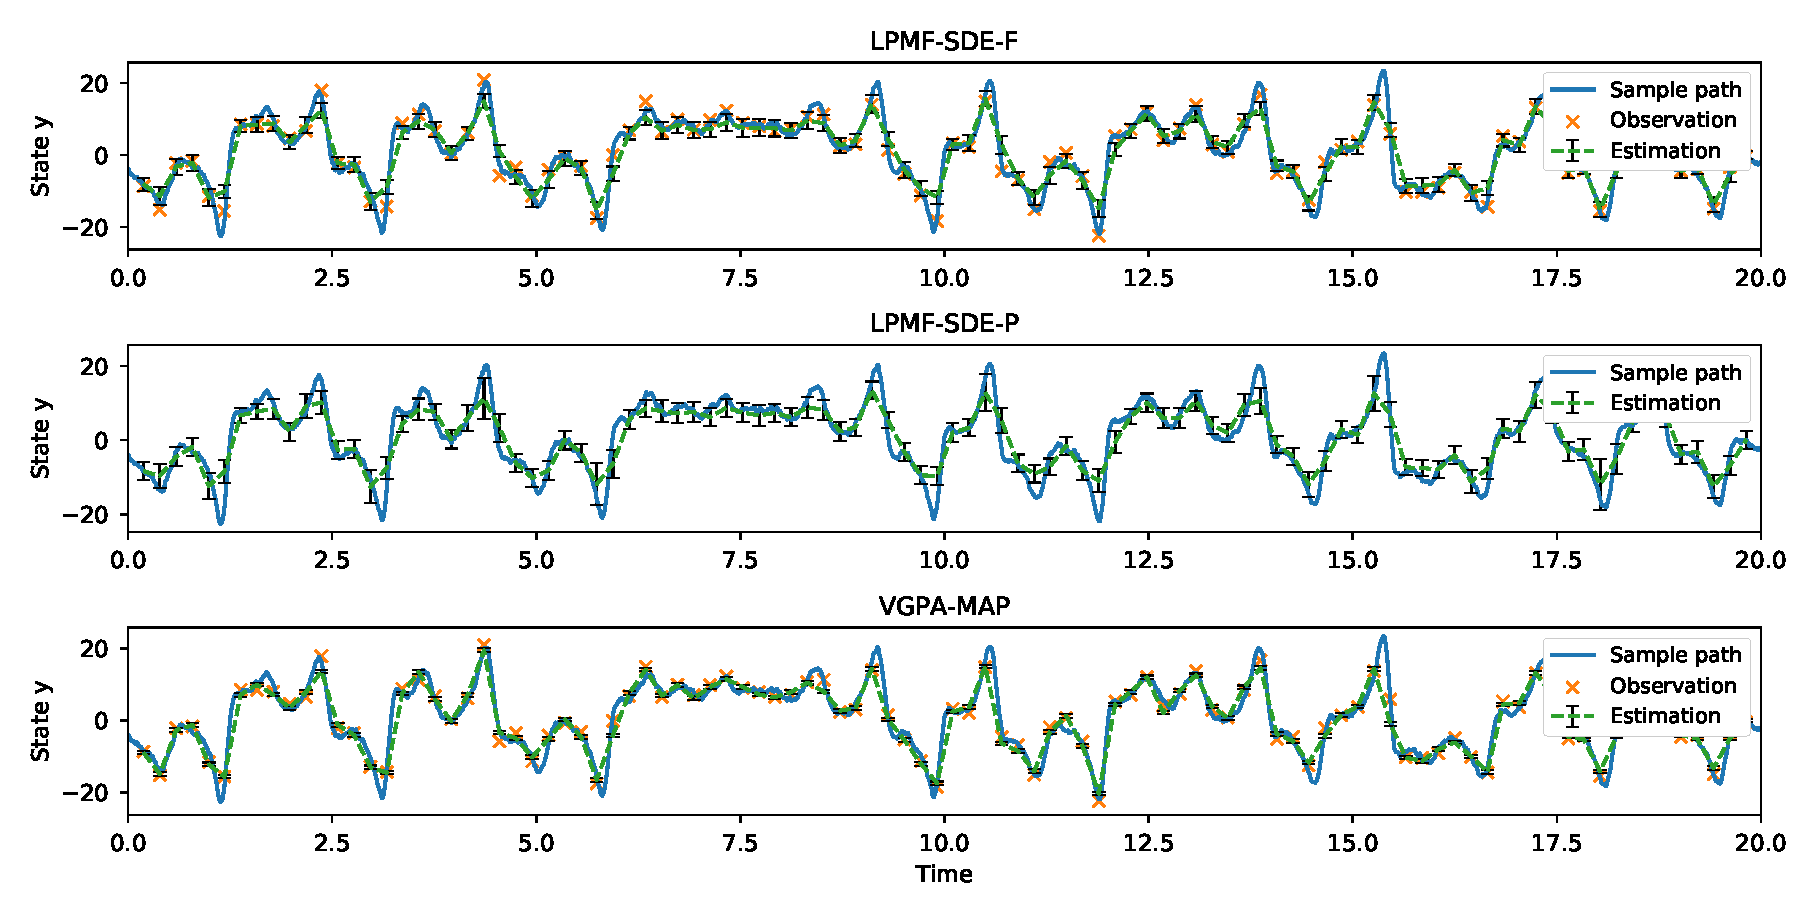
\includegraphics[width=0.95\textwidth]{graphics/lorenz-63-states}
        \label{fig-lorenz-63-states}
    \end{figure}
\end{frame}

\begin{frame}[t]
    \frametitle{State estimation}
    \begin{figure}
        \centering
        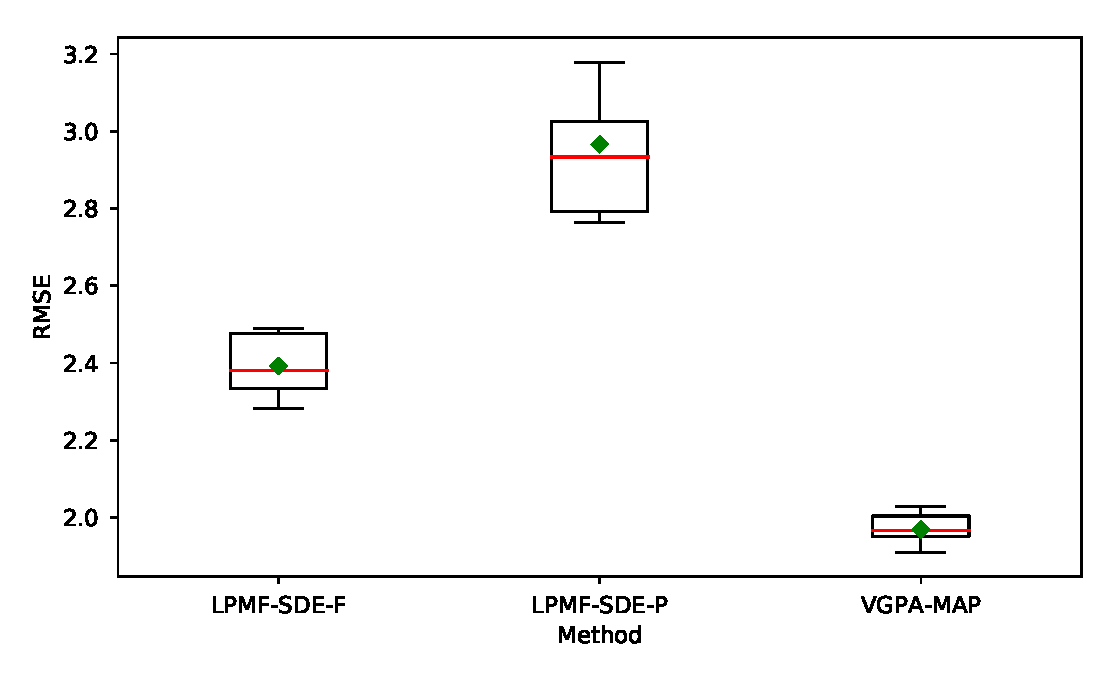
\includegraphics[width=0.7\linewidth]{graphics/lorenz-63-states-boxplot}
        \label{fig-lorenz-63-state-boxplot}
    \end{figure}            
\end{frame}

\begin{frame}[t]
    \frametitle{Parameter estimation}
    \begin{figure}
        \centering
        \begin{subfigure}{0.24\textwidth}
            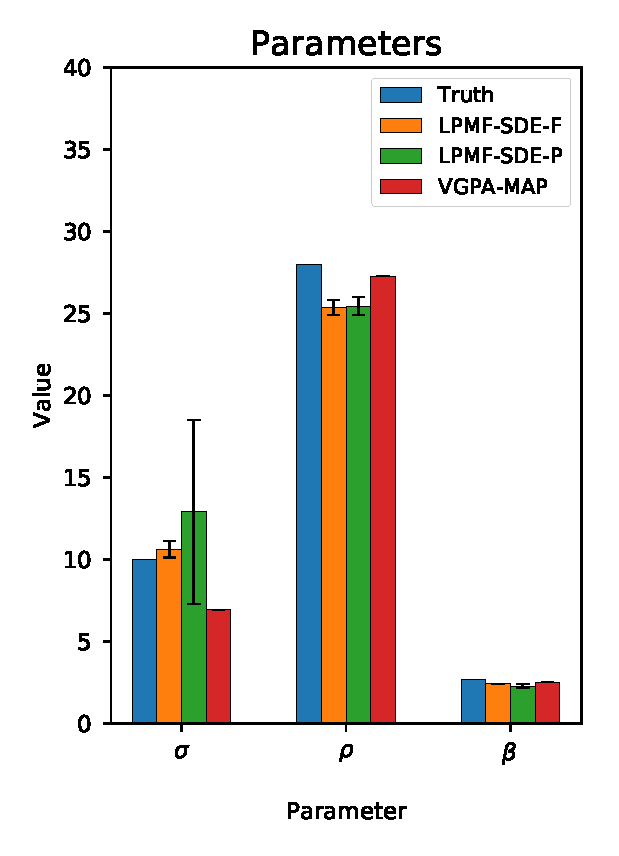
\includegraphics[width=\linewidth]{graphics/lorenz-63-parameters}
            \label{fig-lorenz-63-parameters}
        \end{subfigure}
        \begin{subfigure}{0.24\textwidth}
            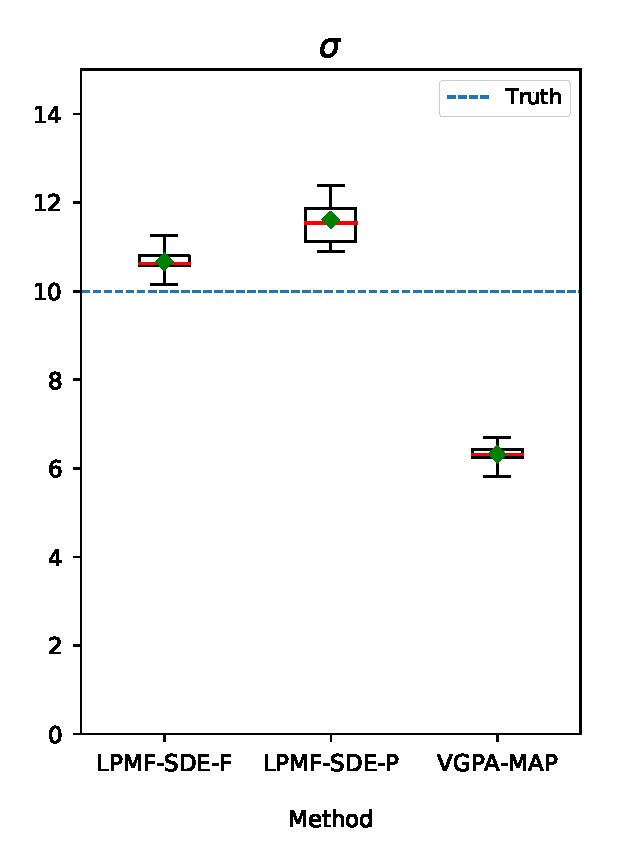
\includegraphics[width=\linewidth]{graphics/lorenz-63-parameters-sigma-boxplot}
            \label{fig-lorenz-63-parameters-sigma-boxplot}
        \end{subfigure}
        \begin{subfigure}{0.24\textwidth}
            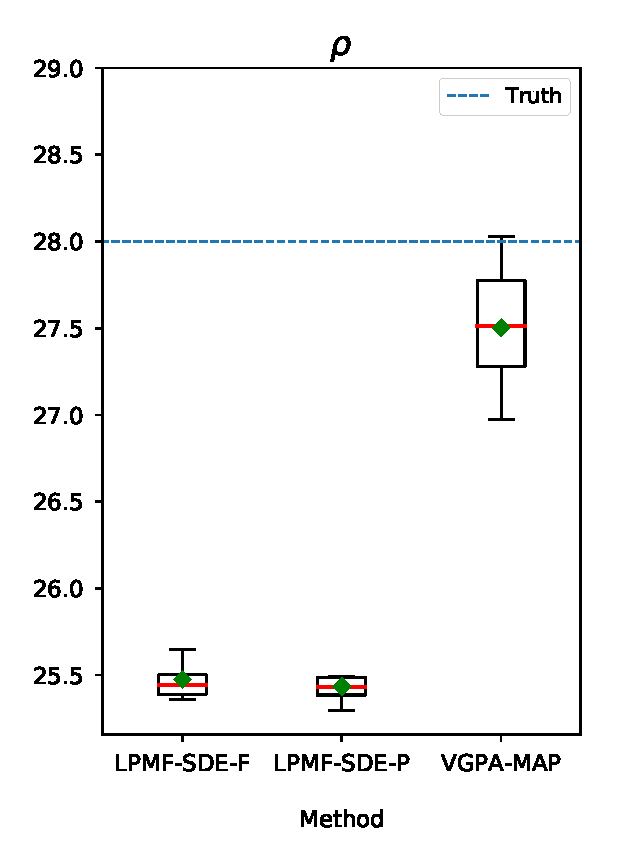
\includegraphics[width=\linewidth]{graphics/lorenz-63-parameters-rho-boxplot}
            \label{fig-lorenz-63-parameters-rho-boxplot}
        \end{subfigure}
        \begin{subfigure}{0.24\textwidth}
            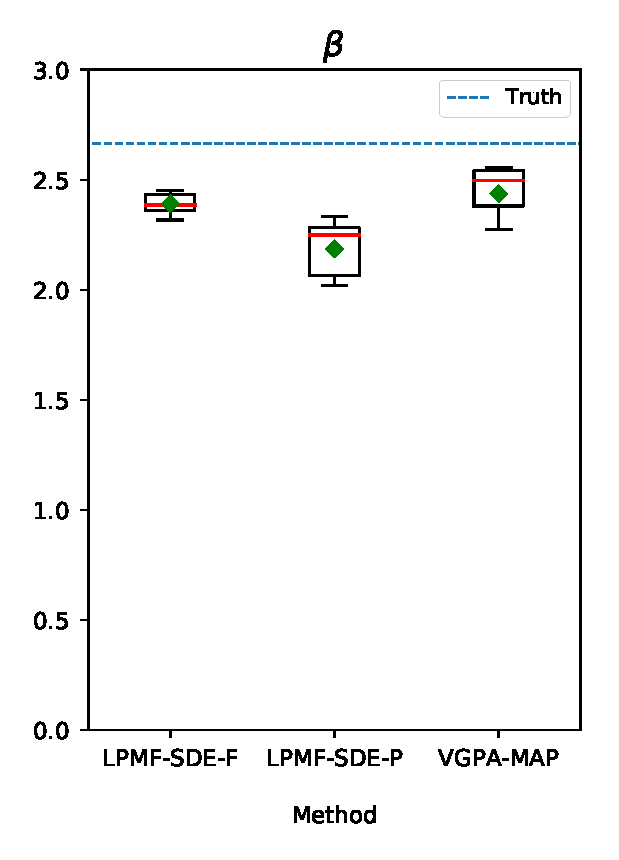
\includegraphics[width=\linewidth]{graphics/lorenz-63-parameters-beta-boxplot}
            \label{fig-lorenz-63-parameters-beta-boxplot}
        \end{subfigure}
        \label{fig-lorenz-63-parameters-group}
    \end{figure}    
\end{frame}

\begin{frame}[t]
    \frametitle{Parameter estimation}
	\begin{figure}
	    \centering
	    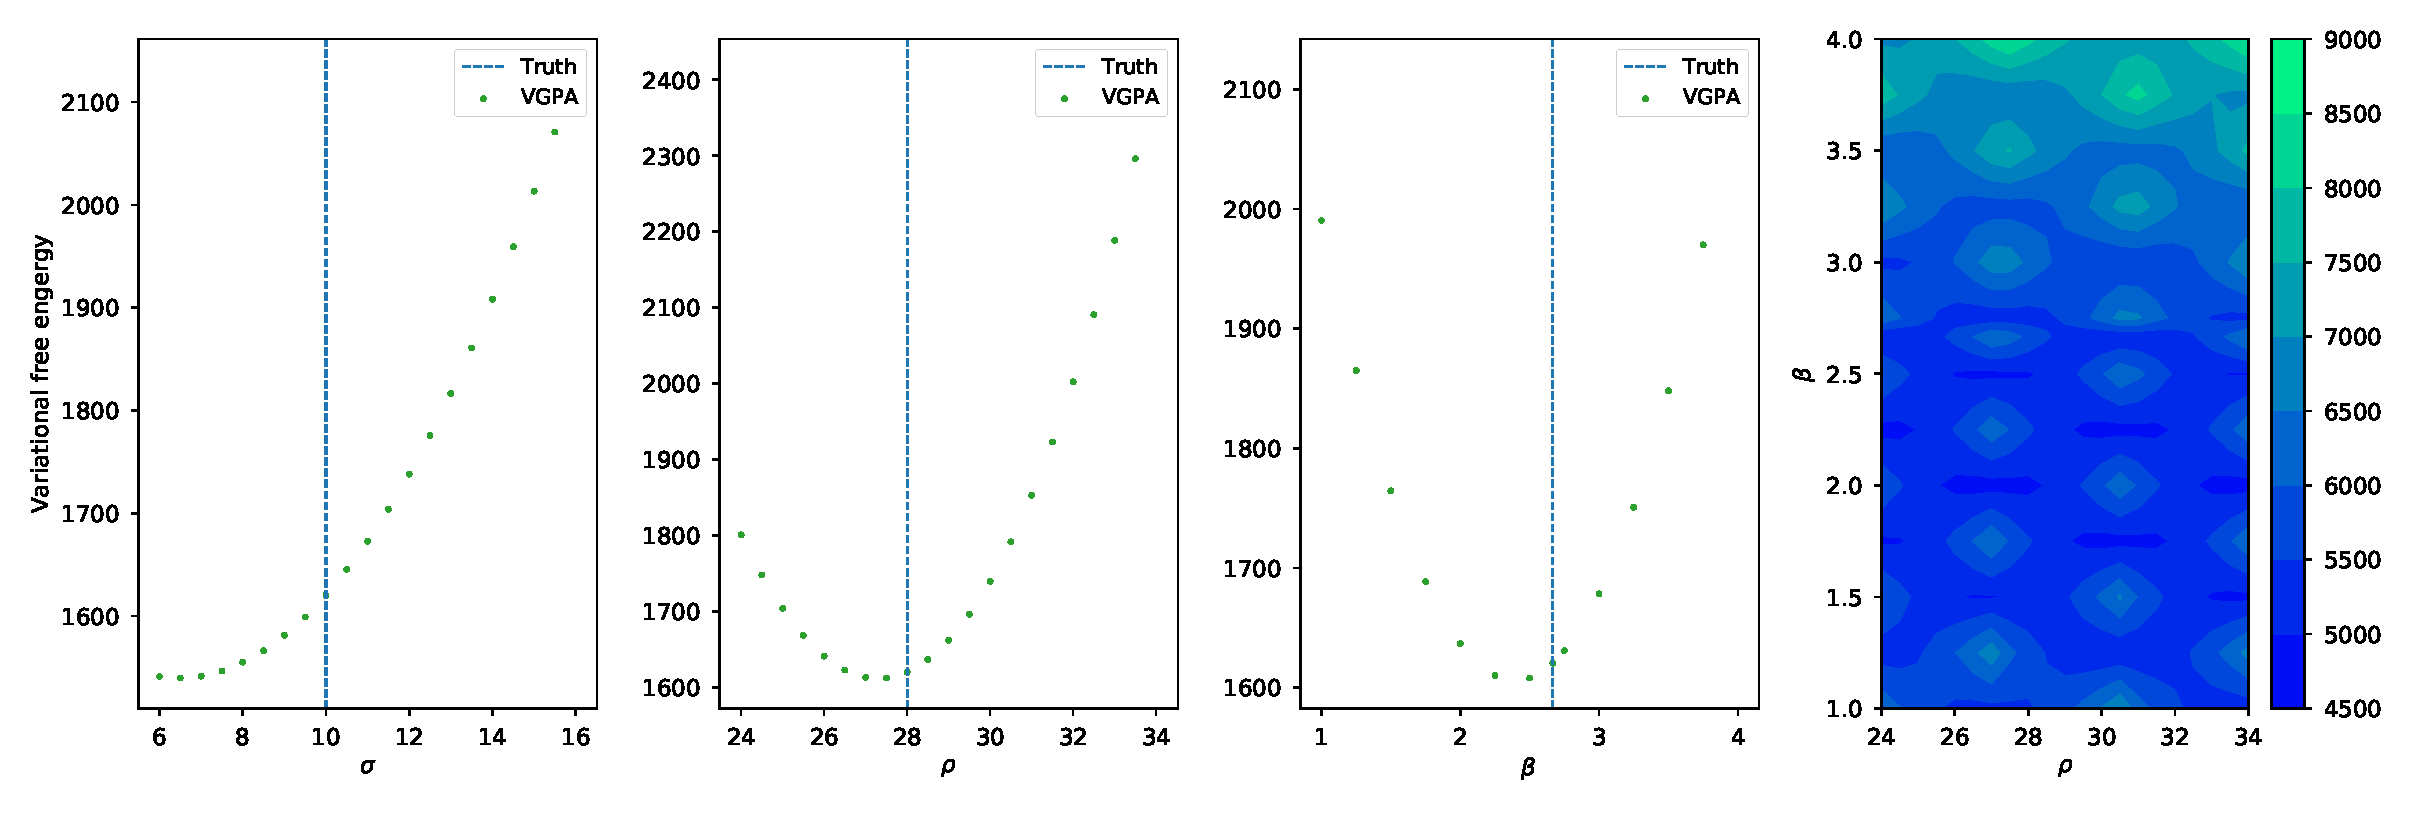
\includegraphics[width=\linewidth]{graphics/lorenz-63-parameters-grid-search}
	    \label{fig-lorenz-63-parameters-grid-search}    
	\end{figure} 
\end{frame}

\begin{frame}[t]
    \frametitle{Runtime performance}
    \begin{figure}
        \centering
        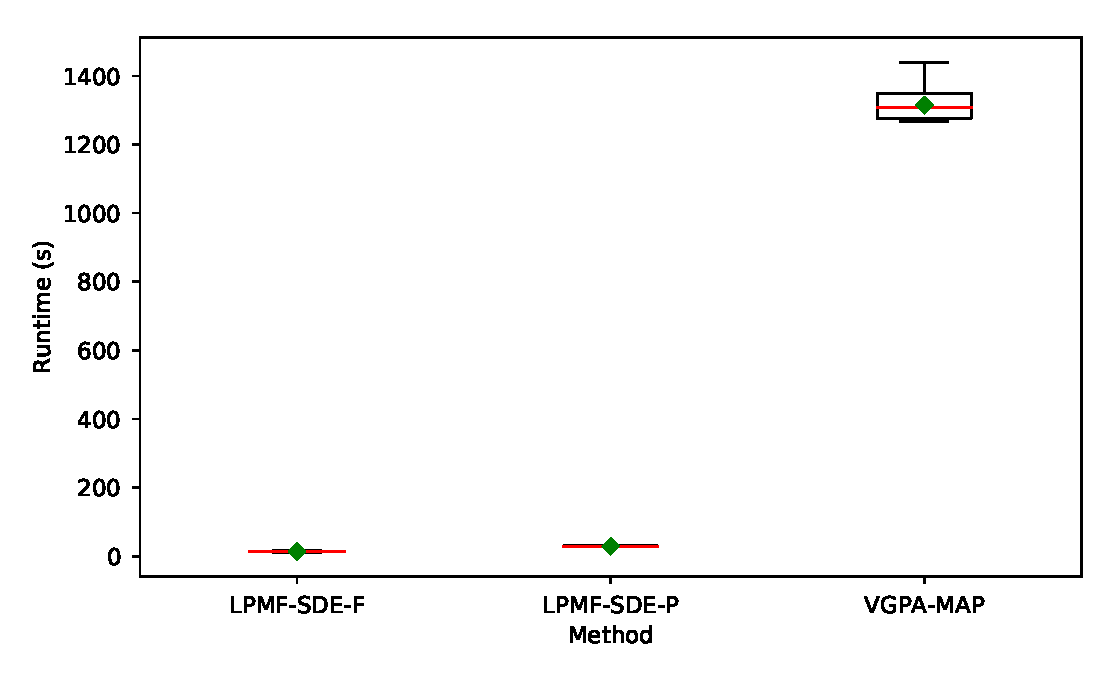
\includegraphics[width=0.7\linewidth]{graphics/lorenz-63-runtime-boxplot}
        \label{fig-lorenz-63-runtime-boxplot}    
    \end{figure}
\end{frame}